\id{ҒТАМР}: 31.23.99

{\bfseries ПОЛИСАХАРИД ПЕН МОНТМОРИЛЛОНИТ БИОНАНОКОМПОЗИТТЕРІНЕ}

{\bfseries КҮМІС НАНОБӨЛШЕКТЕРІН ИММОБИЛИЗАЦИЯЛАУ}

{\bfseries Б.М. Жақып\textsuperscript{\envelope }, Қ.Б. Мусабеков, А.Е. Нурмаханова}

әл-Фараби атындағы Қазақ Ұлттық университеті, Алматы қ., Қазақстан

{\bfseries \textsuperscript{\envelope }}Корреспондент-автор:
\href{mailto:zhakyp.botagoz@mail.ru}{\nolinkurl{zhakyp.botagoz@mail.ru}}

Мақалада табиғи полимерлер мен монтмориллониттен алынған
бионанокомпозиттер құрамына күміс иондарының иммобилизациялану
мүмкіндігі қарастырылған, сонымен қатар, альгин қышқылының натрий тұзы
(Na-ALG), карбоксиметилцеллюлозаның натрий тұзы (Na-КМЦ) және
натриймонтмориллонит (Na-MMT) қоспаларының бионанокомпозиттерінің (BNC)
құрамындағы күміс нанобөлшектерінің (Ag-NPs) суда ісіну кинетикасы,
сондай-ақ, олардан Ag⁺ иондарының бөлініп шығу кинетикасына әсерін
зерттеу нәтижелері берілген. BNC құрамындағы Ag-NPs мөлшерінің
жоғарылауымен оның беріктігі артып, ісінуі 2,5 есеге дейін төмендейтіні
және Ag⁺ иондарының бөлініп шығу кинетикасы жоғарылайтыны көрсетілген.
Бионанокомпозиттердің құрамындағы белсенді заттар мен полимерлерден
басқа, композиттерден күміс иондарының бөлінуіне рН әсері зерттелді.
Ерітіндінің рН жоғарылаған сайын күміс иондарының бөліну дәрежесі де
жоғарылайтыны анықталды. рН мәні 1,2-ден 7,4-ке дейін жоғарылаған сайын,
күміс иондарының бөлініп шығу кинетикасы 3 есеге дейін артты. Зерттеу
нәтижелері отандық монтмориллониттен және арзан, қолжетімді табиғи
полимерлерден биологиялық ыдырайтын, сонымен қатар, биологиялық
қолжетімді композиттерді алуға мүмкіндік береді. Бұл жұмыста
бионанокомпозиттердің құнды қасиеті болып табылатын
Ag\textsuperscript{+} иондарының сулы ерітіндіге ұзақ шығуы үшін
иммобилизация процесін оңтайландырып, «күміс монтмориллониті» және
полисахаридтер негізінде пленкалар алу мүмкіндігі көрсетілді. Мақалада
алынған нәтижелер бионанокомпозиттер өндірісін нақты өнеркәсіптік
өндіріске енгізу мүмкіндігін дәлелдеуге негіз береді.

{\bfseries Түйін сөздер:} күміс нанобөлшектері, бионанокомпозит,
монтмориллонит, полисахарид, күміс иондарының бөлініп шығу кинетикасы,
механикалық беріктілік, ісіну кинетикасы{\bfseries .}

{\bfseries ИММОБИЛИЗАЦИЯ НАНОЧАСТИЦ СЕРЕБРА В БИОНАНОКОМПОЗИТЫ ПОЛИСАХАРИДА
И МОНТМОРИЛЛОНИТА}

{\bfseries Б.М. Жақып\textsuperscript{\envelope }, Қ.Б. Мусабеков, А.Е. Нурмаханова}

Казахский Национальный Университет им. аль-Фараби, Алматы, Казахстан,

e-mail:
\href{mailto:zhakyp.botagoz@mail.ru}{\nolinkurl{zhakyp.botagoz@mail.ru}}

В статье представлены результаты исследований, в ходе которых изучалась
возможность иммобилизации серебра в состав бионанокомпозитов, состоящих
из природных полимеров и монтмориллонита, а также влияние содержания
наночастиц серебра (Ag-NPs) в бионанокомпозитах (BNC) смесей натриевой
соли альгиновой кислоты (Na-ALG), натриевой соли карбоксиметилцеллюлозы
(Na-КМЦ) и натриймонтмориллонита (Na-MMT) на кинетику набухания в воде,
а так же кинетику высвобождения из них ионов Ag⁺. Показано, что с ростом
содержания Ag-NPs в BNC его прочность увеличивается, набухаемость
снижается до 2,5 раз, а кинетика высвобождения ионов Ag⁺ растет. Помимо
содержания бионанокомпозитов, было изучено влияние рН среды на
высвобождение ионов серебра из композитов. Было установлено, что с
увеличением значения рН раствора, степень высвобождения ионов серебра
тоже увеличивалась. То есть при увеличении значения pH от 1,2 до 7,4
кинетика высвобождения ионов серебра увеличивалась до 3 раз. Результаты
исследований дают возможность получать биоразлагаемые, а также
биодоступные композиты из отечественного монтмориллонита и недорогих,
доступных природных полимеров. В данной работе было показано, как можно
получить пленки на основе «серебряного монтмориллонита» и полисахаридов,
оптимизировать процесс иммобилизации для длительного (пролонгированного)
высвобождения в водный раствор ионов Ag\textsuperscript{+}, что делает
их ценными для использования в качестве биоматериалов. Результаты,
полученные в статье дают повод утверждать о возможности внедрения
производство бионанокомпозитов в реальное промышленное производство.

{\bfseries Ключевые слова:} наночастицы серебра, бионанокомпозит,
монтмориллонит, полисахарид, высвобождение ионов серебра, механическая
прочность, кинетика набухания.

IMMOBILIZATION OF SILVER NANOPARTICLES IN BIONANOCOMPOSITES OF
POLYSACCHARIDE AND MONTMORILLONITE

{\bfseries B. M. Zhakyp\textsuperscript{\envelope }, K. B. Мusabekov} {\bfseries A. E.
Nurmakhanova}

al-Farabi Kazakh National university, Almaty, Kazakhstan,

e-mail:
\href{mailto:zhakyp.botagoz@mail.ru}{\nolinkurl{zhakyp.botagoz@mail.ru}}

The article presents the results of the research, in the course of which
the possibility of silver immobilisation into bionanocomposites
consisting of natural polymers and montmorillonite was studied, and the
influence of silver nanoparticles (Ag-NPs) content in bionanocomposites
(BNC) of mixtures of sodium salt of alginic acid (Na-ALG), sodium salt
of carboxymethylcellulose (Na-CMC) and sodium montmorillonite (Na-MMT)
on the kinetics of swelling in water, as well as the kinetics of Ag⁺
ions release from them. It is shown that with the increase of Ag-NPs
content in BNC its strength increases, swelling decreases up to 2,5
times, and the kinetics of Ag⁺ ions release increases. In addition to
the content of bionanocomposites, the influence of the pH of the medium
on the release of silver ions from the composites was studied. It was
found that as the pH value of the solution increased, the degree of
release of silver ions also increased. That is, as the pH value
increased from 1.2 to 7.4, the release kinetics of silver ions increased
up to 3 times. The results of this study provide the possibility of
producing biodegradable as well as bioavailable composites from native
montmorillonite and inexpensive, readily available natural polymers. In
this paper it was shown how films based on "silver montmorillonite" and
polysaccharides can be obtained and the immobilisation process optimised
for prolonged (prolonged) release of Ag\textsuperscript{+} ions into
aqueous solution, making them valuable for use as biomaterials. The
results obtained in the article give reason to assert the possibility of
introducing the production of bionanocomposites into real industrial
production.

{\bfseries Keywords:} nanoparticles of silver, bionanocomposite,
montmorillonite, polysaccharide, silver ions release, mechanical
strength, swelling kinetics.

Кіріспе. Металл күмістің және оның қосылыстарының бактерицидтік
қасиеттері ежелден белгілі. Кішігірім концентрацияларда олар көптеген
бактерияларға зиян келтіреді (650-ден астам патогендік микроорганизмдер
{[}1{]}), бірақ адам жасушалары үшін қауіпсіз {[}2{]}. Күміс
қосылыстарының бірегей микробқа қарсы және вирусқа қарсы қасиеттері
жан-жақты зерттелген. Күміс пен оның қосылыстарының антибиотиктерде жоқ
тамаша ерекшелігі - микроорганизмдердің мутациясын басу қабілеті
{[}3{]}. Күміс пен оның қосылыстарының бұл құнды қасиеті Ag⁺ иондарының
жасушадағы әр түрлі ақуыз объектілерінің көбіне шабуыл жасауымен
байланысты {[}3{]}. Күміс нанобөлшектері оның коллоидты бөлшектеріне
және тіпті Ag⁺ иондарына қарағанда белсендірек екені анықталды {[}4{]}.
Сондықтан күміс нанобөлшектерін дамытуға көп көңіл бөлінеді {[}5{]}.

Металл күмістің бактерицидтік қасиеттері оның баяу тотығуымен және
қоршаған ортаға Ag⁺ иондарының бөлінуімен байланысты. Сондықтан
нанокүміс препараттарын биоцидтік препараттардың арнайы класы ретінде
пайдалану перспективті болып көрінеді {[}3{]}. Олар микроорганизмдермен
максималды жанасуды қамтамасыз ететін жоғары дамыған бетінің арқасында
жоғары бактерияға қарсы тиімділікке ие {[}3{]}. E. coli, V. Cholera, P.
Aeruginosa және Satyphys микроорганизмдеріне олардың өсуінің логарифмдік
фазасында Ag нанобөлшектерінің өлшемдерінің (3-25 нм) әсерін зерттеу
V.Cholera мен P. Aeruginosa күміс нанобөлшектерінің (0, 25, 50, 75, 100
мкг мл‾¹) зерттелген концентрация диапазоны E. coli және Satyphys
қарағанда төзімді екенін, күміс нанобөлшектерінің бактерицидтік әсері
олардың мөлшеріне қатты байланысты - тек жеке диаметрі 10 нм-ден аз Ag⁺
нанобөлшектері бактерицидтік әсерге ие болатынын көрсетті. Бұл
интервалда күміс нанобөлшектерінің 98\% декаэдрлер мен икосаэдрлер болып
табылады, бұл көп қырлыларда көп мөлшерде болатын күміс кристалындағы
{[}6{]} беттер химиялық белсенділікті жоғарылатты.

Күміс нанобөлшектерінің микроорганизмдерге әсер ету механизмі күміс
нанобөлшектерінің бактерия қабырғаларының күкірт және фосфоры бар
аймақтарымен әрекеттесуімен және олардың белсенділігінің жоғалуымен
байланысты {[}3{]}.

Коллоидты күмістің бактерияға қарсы белсенділігі мен одан күміс
иондарының бөліну жылдамдығы арасындағы байланысты анықтау ғалымдарды
айтарлықтай қызықтырады {[}7{]}. Хитозан -- Ag -- поливинипирролидон
(PVP) нанокомпозитінің ерітіндісіне күміс иондарының шығу жылдамдығы
нанобөлшектердің бетінен оксидті қабаттың еру жылдамдығымен және
металдық күмістің тотығу жылдамдығымен анықталатыны атап өтілген.
Монтмориллонит пен күмістің коллоидты бөлшектері бар
бионанокомпозиттерде Ag\textsuperscript{+} иондарының бөліну жылдамдығы
Ag атомдарының диффузия жылдамдығымен және олардың тотығу жылдамдығымен
анықталады {[}8{]}. Құрамында коллоидты күміс бөлшектері бар кальций
альгинаты пленкаларының жоғары бактерицидтік белсенділігі де көрсетілген
{[}9{]}. Жалпы алғанда, полимерлі матрицаларда иммобилизацияланған күміс
иондарының микробқа қарсы белсенділігі жоғары екені айқын болады.
Дегенмен, тасымалдаушы құрамындағы полимер мен минералды компоненттердің
қосылысы күміс иондарының тасымалдаушылармен байланысу механизмінің
әртүрлі болуына байланысты мұндай микробқа қарсы композиттердің қызмет
ету мерзімін ұзартуы мүмкін. Мұндай композиттерді алу {[}10-11{]}
жұмыстарында қарастырылды. Күміс иондарының саз балшықтары бар
композиттерін саздардың пакетаралық кеңістігіне Ag\textsuperscript{+}
иондарын енгізу арқылы да, оларды саз бөлшектерінің бетіне адсорбциялау
арқылы да алуға болатыны көрсетілген; полимерлерді пайдалану олардың
концентрациялары мен арақатынастарын таңдауды талап етеді. Сонымен
қатар, күміс иондарын композиттерінің полимерлермен және саздармен
қасиеттерін мақсатты түрде реттеу үшін осы компоненттердің барлығының
әрекеттесу механизмін, композиттердің ісінуін және олардан
Ag\textsuperscript{+} иондарының бөліну кинетикасын егжей-тегжейлі
зерттеу қажет.

Соңғы жылдары күміс пен оның қосылыстарын құрамында бентонит саздарының
микро- және нанобөлшектері бар композицияларда, атап айтқанда,
монтмориллонитте қолдануға көп көңіл бөлінуде {[}12{]}.

Монтмориллонит қабатты құрылымды, суда ісінеді, катионды алмасуға
қатысады {[}13-14{]}, полимер материалдарының механикалық беріктігін
арттыруға қабілетті, емдік қасиеті бар {[}15{]}.

Соңғы жылдардағы зерттеулер нәтижесіне {[}16-17{]} сәйкес,
монтмориллонит пен күміс негізіндегі композиттерді синтезі мен күміс
иондарының бактерицидтік қасиеттері және осы тақырыптың өзектілігі
дәлелденген. Алайда, аталған жұмыстарда поолимерді матрица ретінде
полиэтилен, поливинил сияқты нашар ыдырайтын полимерлер {[}18{]}
қолданылған.

Ал бионанокомпозиттердің полимерлі матрицасы ретінде қолданылатын натрий
альгинаты мен метилцеллюлоза биоүйлесімді және биологиялық ыдырайтын
болып табылады, бұл бионанокомпозиттің экологиялық тазалығын қамтамасыз
етеді {[}12{]}.

Сонымен қатар, монтмориллонит/хитозан негізіндегі композиттер де
зерттелуде {[}19{]}. Бірақ, бұл композиттерде белсенді заттың, яғни
күмістің ұзақ уақыт бойы бөлініп шығу процессі қарастырылмаған.

Бұл жұмыстың мақсаты -- табиғи полимерлер, күміс нанобөлшектері және
қазақстандық монтмориллонит негізіндегі қолжетімді, биологиялық
ыдырайтын әрі арзан отандық бионанокомпозиттерді синтездеу және олардың
физика-химиялық қасиеттерін зерттеу, күміс иондарының ұзақ уақыт бөлініп
шығатын композиттер алу.

{\bfseries Материалдар мен әдістер.} Осы жұмыста Таган кен орнының 14
горизонтының бентонитінен (Шығыс Қазақстан облысы) алынған натрий
монтмориллониті (Na-MMT), орташа молекулалық салмағы
1,08∙10\textsuperscript{5} («Sigma», АҚШ) альгин қышқылының натрий тұзы
(Na-ALG), орташа тұтқырлықпен карбоксиметилцеллюлозаның натрий тұзы
(Na-КМЦ) («Sigma», АҚШ), МЕМСТ 4460-77 бойынша түйіршіктелген «химиялық
таза» квалификациясы бар кальций хлориді (CaCl\textsubscript{2}),
(«Реакхим», Ресей) глицерин, тазалығы ≥99,0\% («Sigma aldrich», АҚШ).

Күміс нанобөлшектерінің (Ag-NPs) көзі ретінде колларгол фармацевтикалық
препараты қолданылды.

Бионанокомпозиттік пленкалар BNC гидрогелі көлемінде Na-ALG, Na-КМЦ,
CaCl\textsubscript{2}, глицерин, күміс нанобөлшектері Ag-NPs және Na-MMT
макромолекулаларының біркелкі таралуын қамтамасыз ету арқылы алынады
{[}15{]}. Осы мақсатта Na-КМЦ (3\%) және Na-ALG (2\%) сулы ерітінділері
бөлек дайындалды. Содан кейін олар 1:2 қатынасында араластырылды. Бөлек
түрде 1:0,037 қатынасында бентонит пен колларгол (Ag-MMT) қоспасы
дайындалды {[}10{]}. Әрі қарай құрамында 3\%, 6\%, 8\% және 10\% Ag-MMT
(BNC құрамының қатынасы негізінде) бар гидрогель суспензиясы алынды. Ол
үшін магнитті араластырғышта 20 минут араластыра отырып, 1:2
қатынасындағы Na-КМЦ (3\%) және Na-ALG (2\%) қоспасына жоғарыда
көрсетілген концентрацияларға сәйкес келетін Ag-MMT енгізілді.
Пленкалардың серпімділігін қамтамасыз ету үшін ерітіндіге глицерин
(Ag-MMT массасына тең) қосылды, беріктік үшін гидрогельдің жалпы
көлеміне 1:100 қатынасында 1\% CaCl\textsubscript{2} ерітіндісі қосылды.
CaCl\textsubscript{2} және Na-ALG өзара әрекеттесу нәтижесінде ерімейтін
кальций альгинаты түзілді, бұл бионанокомпозиттерге ұзақ уақыт сулы
ерітіндіде ерімеуге және ұзақ уақыт бойы күміс иондарын босатуға
мүмкіндік береді. Осыдан кейін алынған суспензиядан 10 мл диаметрі 85 мм
Петри табақшасына қосылып, 20±2ºС температурада тұрақты салмаққа дейін
кептірілді {[}12{]}.

\emph{Ісіну кинетикасын анықтау}. Бионанокомпозиттердің ісіну
кинетикасын анықтау үшін оның алдын ала аналитикалық таразыда өлшенген
құрғақ үлгісі тазартылған суы бар ыдысқа салынды. 20 °C температурада
120 минут (t) ішінде оның салмағы 5-тен 30 минутқа дейінгі аралықпен
анықталды. BNC кинетикасын анықтау үшін дәлдігі 0,0001 г болатын Kern
аналитикалық таразылары (KERN \& SohnGmbH, Германия) қолданылды.

Полимердің ісіну дәрежесі мына формуламен анықталады:

\(К_{swel} = \frac{m - m_{0}}{m_{0}}\) (1)

mₒ, m -- полимердің ісінуге дейінгі және кейінгі массалары {[}12{]}.

\emph{Пленкалардың беріктігін анықтау.} Пленкалардың соққыға беріктігі
Константа У1-A құрылғысында МЕМСТ 4765-73 сәйкес, пластинаға жүктің
еркін түсуі кезінде пленка деформациясы негізінде, белгілі бір
биіктіктен һ, м. түсетін жүктің потенциалдық энергиясының мәнімен
көрсетілді. Сынақ 20± 0,5ºС және ауаның салыстырмалы ылғалдылығы 65±5\%
жүргізілді. Анықтау кемінде үш рет жүргізілді {[}12{]}.

\emph{Күміс иондарының бөліну кинетикасын анықтау.} Ag⁺ иондарының
бөліну кинетикасы олардың ерітіндідегі концентрациясының өзгеру
жылдамдығымен анықталды

\(F = \frac{C_{t}}{C_{\propto}}\), (2)

мұндағы C\textsubscript{t} және C\textsubscript{∞} - t уақытындағы
Ag\textsuperscript{+} иондарының концентрациясы және мүмкін болатын
максималды концентрациясы. Бионанокомпозиттерден күміс иондарының бөліну
кинетикасын анықтау үшін аналитикалық таразыда өлшенген 0,1 г құрғақ
үлгі 30 мл тазартылған су және физикалық ерітіндісі бар ыдыстарға
салынды. Ag⁺ иондарының концентрациясы Agilent 8453E УК
спектрофотометрін (Agilent Technologies Deutschland GmBH, Германия)
пайдалана отырып, 405 нм {[}14{]} толқын ұзындығында 15 тәулік бойы
анықталды. Күміс иондарының бөліну кинетикасының ортаның рН мәніне
тәуелділігін анықтау үшін бұл талдау 3 түрлі рН 1,2; 5,0; және 7,4
физикалық ерітінділерде жүргізілді.

{\bfseries Нәтижелер мен талқылау.} Бионанокомпозиттердің сумен әрекеттесуі
осы материалдарды практикалық қолдану салаларын анықтайтын маңызды
қасиеттердің бірі болып табылады. 1-суретте бионанокомпозиттердің судағы
ісіну кинетикасы көрсетілген. Қарастырылып отырған бионанокомпозиттер
өте тез ісінетінін атап өтуге болады - тепе-теңдік мәндері
(К\textsubscript{swel}) \textasciitilde30 минутта орнатылады. Сонымен
қатар, бионанокомпозиттегі Ag-MMT мөлшерінің жоғарылауымен олардың
ісінуі төмендейді - Ag-MMT мөлшері 3\%-дан (BNC-1) 10\%-ға (BNC-4)
жоғарылағанда, тепе-теңдік ісіну коэффициентінің мәні
(К\textsubscript{swel}) \textasciitilde2.5 есе төмендейді.

\begin{figure}[H]
	\centering
	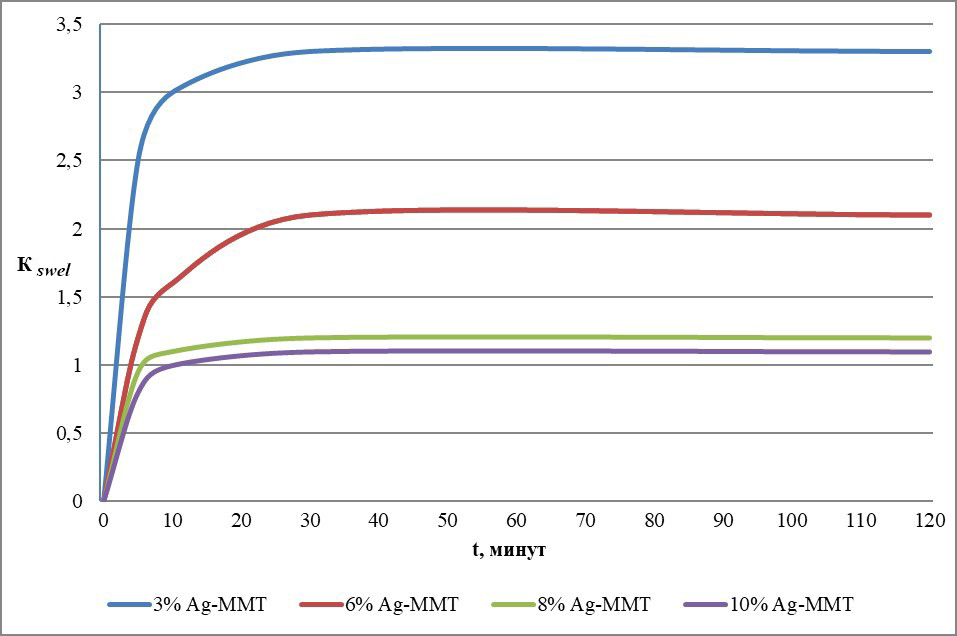
\includegraphics[width=0.8\textwidth]{media/chem/image14}
	\caption*{}
\end{figure}


{\bfseries 1-сурет - Бионанокомпозиттердің судағы ісіну кинетикасы, t=20ºС}

Алынған құрылымның қасиеттері, атап айтқанда, тордың тығыздығы, оның
механикалық беріктігі және ол арқылы дәрілік заттарды тасымалдау
кинетикасы, оның құрамындағы Na-MMT нанобөлшектерінің мөлшерімен
анықталады.

Бұл күмістің амин топтары және гидроксил топтары бар хелат
қосылыстарының түзілуіне байланысты үш өлшемді BNC торында қосымша тігіс
түйіндерінің пайда болуына байланысты болуы мүмкін {[}20{]}. Байқалған
құбылысты түсіндіру үшін ион алмастырғыш шайырлардың гидратация
механизмі туралы қазіргі заманғы өкілдерге жүгінуге болады, оларда әлсіз
қышқылды иониттерде сияқты функционалды -COO- топтарының болуына
байланысты аталған шайырлар сияқты бионанокомпозиттер деп тануға болады.

Ионалмастырғыштарды сумен гидратациялау механизмін ИҚ-спектроскопия
арқылы зерттеу негізінде құрылған Цундельдің идеялары бойынша бұл
процесс су молекулаларының қарсы ионмен, біздің жағдайда Na-КМЦ
құрамындағы Na\textsuperscript{+} және Ag-MMT бар бионанокомпозиттік
пленкадағы Ag\textsuperscript{+} иондарымен әрекеттесуінен басталады.
Қарсы ион бірінші су молекуласын бекітіп, полимер матрицасында (-COO-)
бекітілген топтан біршама алыстайды. Кейінгі гидратация қабаттары қарсы
ион мен бекітілген топтың арасында да, айналасында да түзіледі. Қарсы
ион радиусы ұлғайған сайын ион зарядының тығыздығының төмендеуіне
байланысты оның гидратациясы әлсірейді.

Осылайша, Na-КМЦ-ден BNC-ге өткенде пленкалардың ісінуінің төмендеуін
Na\textsuperscript{+} иондарынан аз гидратталған Ag\textsuperscript{+}
иондарының мөлшерінің жоғарылауымен түсіндіруге болады.

Екінші жағынан, бионанокомпозитті құрылымдайтын монтмориллониттің
коллоидты бөлшектері де оның ісінуін азайтады деп болжауға болады.
Сондықтан құрамында Ag-MMT коллоидты бөлшектері бар
бионанокомпозиттердің байқалған ісінуінің төмендеуін осы екі әсердің
суперпозициясы ретінде қарастыруға болады.

BNC тәжірибеде, атап айтқанда, тамақ өнімдерін орау материалы ретінде,
биоқолғаптар ретінде және т.б. пайдаланылған кезде, олардың механикалық
беріктігінің маңызға зор. Осыған байланысты BNC құрамының олардың
соққыға беріктігіне әсері зерттелді (1-кесте).

{\bfseries 1-кесте- Бионанокомпозиттердің соққыға беріктігі}

% \begin{longtable}[]{@{}
%   >{\raggedright\arraybackslash}p{(\columnwidth - 4\tabcolsep) * \real{0.0600}}
%   >{\raggedright\arraybackslash}p{(\columnwidth - 4\tabcolsep) * \real{0.4712}}
%   >{\raggedright\arraybackslash}p{(\columnwidth - 4\tabcolsep) * \real{0.4689}}@{}}
% \toprule\noalign{}
% \begin{minipage}[b]{\linewidth}\raggedright
% №
% \end{minipage} & \begin{minipage}[b]{\linewidth}\raggedright
% Бионанокомпозит
% \end{minipage} & \begin{minipage}[b]{\linewidth}\raggedright
% Соққыға беріктігі, Н∙м
% \end{minipage} \\
% \midrule\noalign{}
% \endhead
% \bottomrule\noalign{}
% \endlastfoot
% 1 & BNC-1 & 2750 \\
% 2 & BNC-2 & 2870 \\
% 3 & BNC-3 & 2950 \\
% 4 & BNC-4 & 3030 \\
% \end{longtable}

Алынған нәтижелерді талдау, қарастырылып отырған BNC пленкаларының
механикалық беріктігі олардағы Ag-NPs мөлшерінің жоғарылауымен жоғарылау
тенденциясын көрсетеді. Бұл нәтижелерді жоғарыда аталған BNC торларының
тығыздығымен түсіндіруге болады.

Биананокомпозиттерді қолданудың дәстүрлі бағыттарының бірі, олардың ұзақ
уақыт бойы шығарылуын қамтамасыз ету үшін, құрамына бактерицидтік
препараттарды иммобилизациялау болып табылады.

Коллоидты химиялық көзқарас тұрғысынан бионанокомпозиттер полимердің
үздіксіз дисперсиялық ортасынан және дисперсті фазадан -- толтырғыштың
коллоидты бөлшектерінен -- бұл жағдайда Ag-MMT бөлшектерінен тұратын
толтырылған полимерлі материалдардың бір түрі болып табылады. Мұндай
жүйелердің реологиялық, оның ішінде механикалық қасиеттері, полимердің
адсорбциялық қабаты арқылы толтырғыш бөлшектерінің бір-бірімен
коагуляциялық құрылымының түзілуімен анықталады. Бұл процесс
макромолекула сегменттерінің Гиббс бос энергиясы артық толтырғыш
бөлшектердің бетімен әрекеттесуі нәтижесінде полимердің адсорбциялық
қабатының күшеюімен жүреді. Бұл ұстаным академик П.А. Ребиндер мен оның
әріптестері белгілеген құрылымсыз полимер ерітіндісінде толтырғыш
бөлшектердің - белсенді титан диоксиді мен бентонит сазының үздіксіз
құрылымдық торын қалыптастыруда расталды.

Толтырылған полимерлердің механикалық қасиеттерінің олардағы
толтырғыштың құрамына өте тәуелділігімен сипатталады. Бұл толтырғыш
концентрациясының жоғарылауымен толтырғыш бөлшектердің бетіндегі
макромолекулалардың адсорбциялық қабаттарының үлесінің өзгеруіне
байланысты {[}21{]}. Толтырғыштың дисперсия дәрежесінің жоғарылауымен
толтырылған полимерде кеңістіктік коагуляциялық құрылым пайда болатын
толтырғыштың минималды концентрациясы төмендейді.

Жоғарыда атап өтілгендей, бионанокомпозиттерде иммобилизацияланған күміс
иондарының бөліну кинетикасы негізінен осы бөлшектердің суды сіңіруімен
анықталады. Осыған байланысты, бұл жұмыста бионанокомпозиттерден
Ag\textsuperscript{+} иондарының бөлінуі зерттелді. 2-3-суреттерден
Ag\textsuperscript{+} иондарының бөлінуі жылдам емес, кинетикалық
процесс екені анық көрінеді. 15 тәулік бойы әртүрлі рН мәндерінде,
сондай-ақ, BNC құрамындағы Ag-MMT мөлшеріне байланысты
бионанокомпозиттерден белсенді заттың бөліну дәрежесі біртіндеп өсті. Он
бес тәулікте бұл процесс әлі біткен жоқ. Ортаның рН жоғарылаған сайын
Ag\textsuperscript{+} иондарының бөлінуі артады (3-сурет).

2-суретте BNC-дан Ag⁺ иондарының бөліну кинетикасы көрсетілген. Ag-NPs
мөлшерінің жоғарылауымен, BNC ісінуінің төмендеуіне қарамастан,
процестің кинетикасы артатынын атап өтуге болады. Мұны қарастыратын BNC
құрылымында Ag⁺ иондарының диффузиясы үшін жеткілікті мәні бар торлардың
түзілуімен түсіндіруге болады.

\begin{figure}[H]
	\centering
	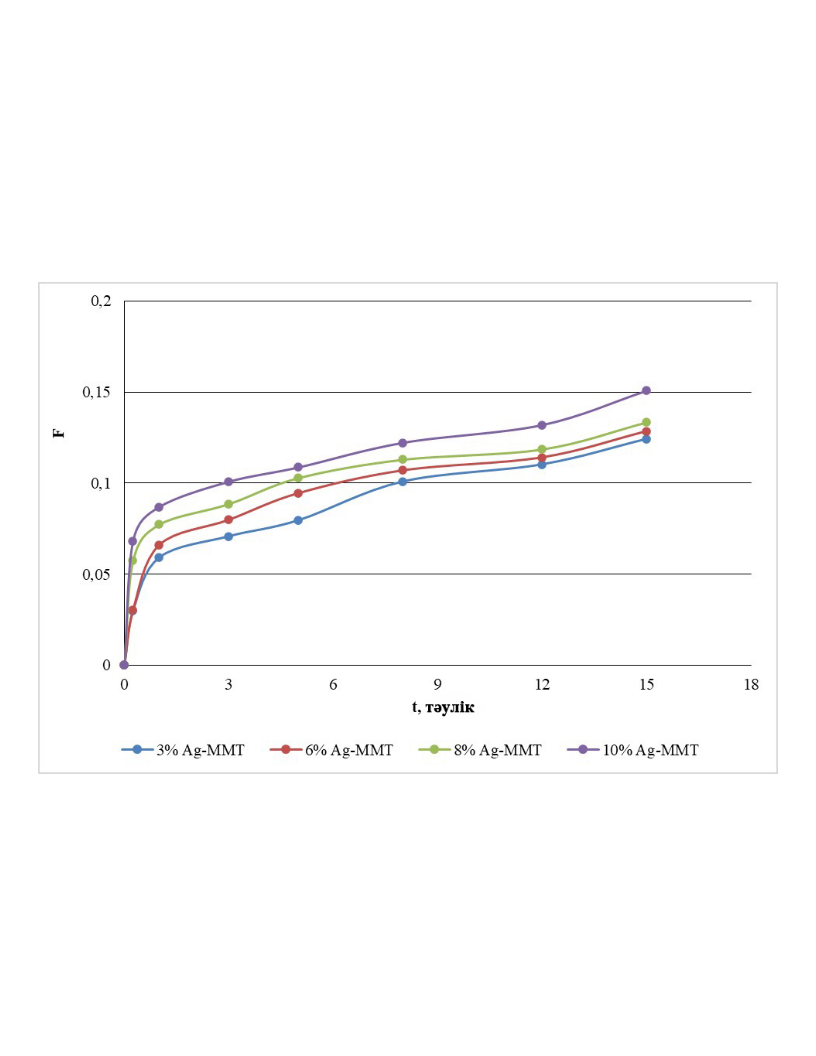
\includegraphics[width=0.8\textwidth]{media/chem/image15}
	\caption*{}
\end{figure}


{\bfseries 2-сурет- BNC-тен Ag\textsuperscript{+} иондарының судағы бөліну
кинетикасы, t=20ºС}

\begin{figure}[H]
	\centering
	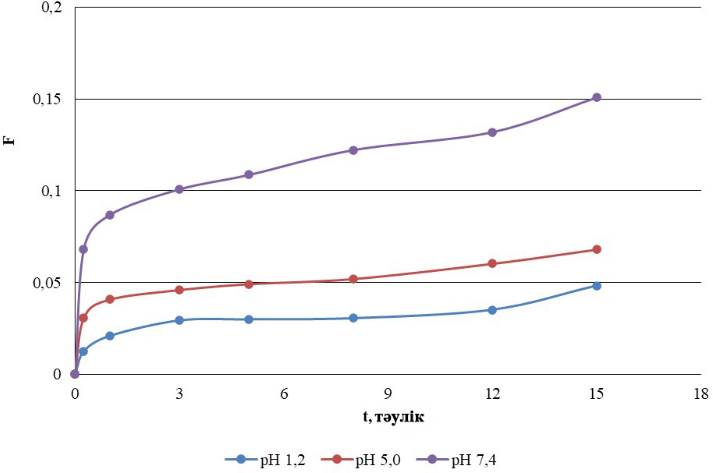
\includegraphics[width=0.8\textwidth]{media/chem/image16}
	\caption*{}
\end{figure}


{\bfseries 3-сурет - Әртүрлі рН мәндеріндегі BNC-ден Ag\textsuperscript{+}
иондарының физикалық ерітіндідегі бөліну кинетикасы, t=20ºС}

Осыған ұқсас нәтижелер {[}22{]} жұмысында бионанокомпозиттердің су
сіңіруін және олардан Ag\textsuperscript{+} иондарының бөліну
кинетикасын зерттеу кезінде алынған. Композиттегі Ag-MMT мөлшері
неғұрлым жоғары болса, соғұрлым Ag\textsuperscript{+} иондары тезірек
бөлінеді. Келтірілген жұмыста Ag\textsuperscript{+} иондары BNC-ден
бөлінген кезде оң зарядталған полимерлі матрицада диффузияланатынын
ескерген жөн. Біздің қарастырып отырған альгин қышқылының натрий тұзына
және карбоксиметилцеллюлозаның натрий тұзына негізделген BNC-ден
Ag\textsuperscript{+} иондары теріс зарядталған полимерлі ортада
диффузияланады. Бұл жағдайда ион алмасу процесінің өтуін жоққа шығаруға
болмайды. Демек, осы жұмыста зерттелген BNC-дан Ag\textsuperscript{+}
иондарының бөліну кинетикасы аталған {[}22{]} процесстен ерекшеленуі
керек.

{\bfseries Қорытынды.} Микробқа қарсы, биоцидтік препараттар мен коллоидты
күміс негізіндегі өнімдердің ассортиментін кеңейту үшін коллоидты күміс
бөлшектері қабатталған монтмориллонит силикаты құрылымында
иммобилизацияланды.

Альгин қышқылының натрий тұзы, карбоксиметилцеллюлозаның натрий тұзы,
күміс нанобөлшектері Ag-NPs, кальций хлориді, глицерин және натрий
монтмориллониті Na-MMT қоспалары негізінде жаңа бионанокомпозиттердің
пленкалары алынды. Құрамында Ag-NPs жоғарылаған сайын пленкалардың
механикалық беріктігі артып, судағы ісінуі, керісінше, төмендейтіні
анықталды. Бұл бионанокомпозиттердің полимерлік торларының тығыздалуына
байланысты болуы мүмкін. Бионанокомпозиттерден Ag⁺ иондарының бөліну
кинетикасы негізінен оның осы BNC құрамындағы мөлшерімен, Ag-NPs
мөлшерінің жоғарылауымен, сондай-ақ, қоршаған ортаның рН мәнінің
жоғарылауымен анықталады. Бұл Ag⁺ иондарының диффузиясы үшін
бионанокомпозиттерде өлшемдері жеткілікті болатын полимерлік торлардың
пайда болуын көрсетеді.

Осылайша, белсенді заттардың, яғни күміс иондарының, реттеуге келетін
және ұзақ бөлініп шығарылатын бионанокомпозиттерді синтездеуге болады.

Алынған нәтижелер дәрілік, биоцидтік, бактерицидтік препараттардың,
биологиялық ыдырайтын, биоүйлесімді, биополимерлі матрицаларын және
тамақ өнімдеріне, көкөністер мен жемістерге арналған қаптамаларды
жобалау үшін пайдалы болуы мүмкін.

\emph{{\bfseries Қаржыландыру.}} Бұл зерттеуді Қазақстан Республикасы Ғылым
және жоғары білім министрлігінің Ғылым комитеті (Грант № AP19677207)
қаржыландырды.

{\bfseries Әдебиеттер}

\begin{enumerate}
\def\labelenumi{\arabic{enumi}.}
\item
  Pessanha N.F.N., Coelho G.L.V. Study on the production of
  silver/modified clay nanocomposites // Mater. Res. Soc. Symp. Proc. --
  2013. -- Vol. 1547, -- P. 167--172.
  DOI:\href{http://dx.doi.org/10.1557/opl.2013.565}{10.1557/opl.2013.565}
\item
  K.I. Baterseh. Anomaly and correlation of killing in the therapeutic
  properties of silver (I) chelation with glutamic and tartaric acids //
  Journal of Antimicrobial Chemotherapy -- 2004 -- Vol. 54 -- P.
  546--548. DOI: 10.1093/jac/dkh349
\item
  Ю. А. Крутяков, А.А.Кудринский, А.Ю. Оленин, Г.В.Лисичкин. Синтез и
  свойства наночастиц серебра: достижения и перспективы.// Успехи химии.
  -- 2008. -- T. 77, №3. -- С.242-269.
  \href{https://doi.org/10.1070/RC2008v077n03ABEH003751}{DOI:10.1070/RC2008v077n03ABEH003751}
\item
  Balachandran Y.L. et al. Differently Environment Stable Bio-Silver
  Nanoparticles: Study on Their Optical Enhancing and Antibacterial
  Properties // PLoS One. -- 2013. -- Vol. 8, № 10. -- P. 1--14.
  DOI:10.1371/journal.pone.0077043
\item
  О.Я. Урюпина, Е. К. Уродкова, Е. С. Жаворонок, В. В. Высоцкий, И. Н.
  Сенчихин. Синтез монодисперсных наночастиц серебра в растворах
  хитозана // Коллоидный журнал. -- 2019. -- T. 81, № 2. -- С. 263-267.
  DOI: 10.1134/S0023291219020174
\item
  D.W. Hatchett, H.S. White. Electrochemistry of Sulfur Adlayers on the
  Low-Index Faces of Silver. // The Journal of Physical Chemistry. --
  1996 -- Vol. 1006, №28. -- P. 9854--9859.
\item
  Wang, B., Liu, X., Ji, Y., Ren, K., \& Ji, J. (2012). Fast and
  long-acting antibacterial properties of
  chitosan-Ag/polyvinylpyrrolidone nanocomposite films. // Carbohydrate
  Polymers. -- 2012.-- Vol. 90. -- P. 8--15. DOI:
  10.1016/j.carbpol.2012.03.080
\item
  Sotiriou, G. A., Meyer, A., Knijnenburg, J. T. N., Panke, S., \&
  Pratsinis, S. E. Quantifying the origin of released Ag+ ions from
  nanosilver // Langmuir. -- 2012. -- Vol. 23. -- P. 15929--15936. DOI:
  10.1021/la303370d
\item
  Ю.Л. Буркова, И.А. Беленёва, Ю.А. Щипунов. Бактерицидные пленки
  альгината натрия с наноразмерными частицами серебра // Коллоидный
  журнал. -- 2015. -- Т. 77, №6. -- С. 714-722.
\item
  de Azeredo, H. M. C. Antimicrobial nanostructures in food packaging.
  // Trends in Food Science \& Technology. -- 2013 -- Vol. 30. -- P.
  56--69. DOI: 10.1016/j.tifs.2012.11.006
\item
  Kamyar Shameli, Mansor Bin Ahmad, Wan Md Zin Wan Yunus, Abdolhossein
  Rustaiyan, Nor Azowa Ibrahim, Mohsen Zargar, Yadollah Abdollahi. Green
  synthesis of silver/montmorillonite/chitosan bionanocomposites using
  the UV irradiation method and evaluation of antibacterial activity //
  International Journal of Nanomedicine -- 2010 -- Vol.5. -- P.
  875--887. DOI: 10.2147/IJN.S13632
\item
  Shameli K. et al. Synthesis and characterization of
  silver/montmorillonite/chitosan bionanocomposites by chemical
  reduction method and their antibacterial activity. // Int. J.
  Nanomedicine. -- 2011. -- Vol. 6. -- P. 271--284.
  DOI:\href{http://dx.doi.org/10.2147/IJN.S16043}{10.2147/IJN.S16043}
\item
  Mishra R.K. et al. Antimicrobial and in vitro wound healing properties
  of novel clay based bionanocomposite films // J. Mater. Sci. Mater.
  Med. -- 2014. -- Vol. 25, № 8. -- P. 1925--1939.
  DOI:\href{http://dx.doi.org/10.1007/s10856-014-5228-y}{10.1007/s10856-014-5228-y}
\item
  Alcântara A.C.S. et al. Effective intercalation of zein into
  Na-montmorillonite: Role of the protein components and use of the
  developed biointerfaces // Beilstein J. Nanotechnol. -- 2016. -- Vol.
  7, № 1. -- P. 1772--1782. DOI:10.3762/bjnano.7.170
\item
  Makwana D. et al. Characterization of Agar-CMC/Ag-MMT nanocomposite
  and evaluation of antibacterial and mechanical properties for
  packaging applications // Arab. J. Chem. -- 2020. -- Vol. 13, № 1. --
  P. 3092--3099. DOI: 10.1016/j.arabjc.2018.08.017
\item
  Quang Lich Nguyen, Dai Vuong Le, Anh N. Phan, and Van Duy Nguyen.
  Synthesis of Biodegradable and Antimicrobial Nanocomposite Films
  Reinforced for Coffee and Agri-Food Product Preservation // ACS Omega
  -- 2023 -- Vol. 8, №45. -- P. 42177-42185. DOI:
  10.1021/acsomega.3c04017
\item
  Seok-In Hong, Long-Feng Wang, Jong-Whan Rhim. Preparation and
  characterization of nanoclays-incorporated polyethylene/thermoplastic
  starch composite films with antimicrobial activity // Food Packaging
  and Shelf Life -- 2022 -- Vol. 31 -- P. 100784.
  https://doi.org/10.1016/j.fpsl.2021.100784
\item
  Ekta B. Jadhav, Mahipal Singh Sankhla, Rouf Ahmad Bhat, D.S. Bhagat.
  Microplastics from food packaging: An overview of human consumption,
  health threats, and alternative solutions // Environmental
  Nanotechnology, Monitoring \& Management -- 2021 -- Vol. 16 -- P.
  100608. https://doi.org/10.1016/j.enmm.2021.100608
\item
  Yang K, Shen L, Zhang L, Sun W, Zou Y, Ren Y, Zeng R. Antibacterial
  Activity and Biocompatibility of Ag-Montmorillonite/Chitosan Colloidal
  Dressing in a Skin Infection Rat Model: An In Vitro and In Vivo Study
  // J Funct Biomater -- 2023 -- Vol. 14, №9 . -- P. 470. doi:
  10.3390/jfb14090470.
\item
  Alba M.D. et al. Bionanocomposites based on chitosan intercalation in
  designed swelling high- charged micas // Sci. Rep. -- 2019. -- Vol. 9,
  № 1. -- P. 1--9. DOI:10.1038/s41598-019-46495-z
\item
  Плотникова Л.В., Успенская М.В. Игнатьева Ю.А. Модификация
  обогащенного бентонита ионами серебра // Сборник научных трудов по
  итогам международной научно-практической конференции № 1. -- г.
  Тюмень, 2016. -- С. 48-51.
\item
  Lavorgna M. et al. MMT-supported Ag nanoparticles for chitosan
  nanocomposites: Structural properties and antibacterial activity //
  Carbohydr. Polym. Elsevier Ltd. -- 2014. -- Vol. 102, № 1. -- P.
  385--392. ~DOI:
  \href{https://doi.org/10.1016/j.carbpol.2013.11.026}{10.1016/j.carbpol.2013.11.026}
\end{enumerate}

{\bfseries References}

\begin{enumerate}
\def\labelenumi{\arabic{enumi}.}
\item
  Pessanha N.F.N., Coelho G.L.V. Study on the production of
  silver/modified clay nanocomposites // Mater. Res. Soc. Symp. Proc. --
  2013. -- Vol. 1547, -- P. 167--172. DOI:10.1557/opl.2013.565
\item
  K.I. Baterseh. Anomaly and correlation of killing in the therapeutic
  properties of silver (I) chelation with glutamic and tartaric acids //
  Journal of Antimicrobial Chemotherapy -- 2004 -- Vol. 54 -- P.
  546--548. DOI: 10.1093/jac/dkh349
\item
  Yu. A. Krutyakov, A.A.Kudrinskii, A.Yu. Olenin, G.V.Lisichkin. Sintez
  i svoistva nanochastits serebra: dostizheniya i perspektivy.// Uspekhi
  khimii. -- 2008. -- T. 77, №3. -- S.242-269.
  \href{https://doi.org/10.1070/RC2008v077n03ABEH003751}{DOI:10.1070/RC2008v077n03ABEH003751}
  {[}in Russian{]}
\item
  Balachandran Y.L. et al. Differently Environment Stable Bio-Silver
  Nanoparticles: Study on Their Optical Enhancing and Antibacterial
  Properties // PLoS One. -- 2013. -- Vol. 8, № 10. -- P. 1--14.
  DOI:10.1371/journal.pone.0077043
\item
  O.Ya. Uryupina, E. K. Urodkova, E. S. Zhavoronok, V. V. Vysotskii, I.
  N. Senchikhin. Sintez monodispersnykh nanochastits serebra v
  rastvorakh khitozana // Kolloidnyi zhurnal. -- 2019. -- T. 81, № 2. --
  S. 263-267. DOI: 10.1134/S0023291219020174 {[}in Russian{]}
\item
  D.W. Hatchett, H.S. White. Electrochemistry of Sulfur Adlayers on the
  Low-Index Faces of Silver. // The Journal of Physical Chemistry. --
  1996 -- Vol. 1006, №28. -- P. 9854--9859.
\item
  Wang, B., Liu, X., Ji, Y., Ren, K., \& Ji, J. (2012). Fast and
  long-acting antibacterial properties of
  chitosan-Ag/polyvinylpyrrolidone nanocomposite films. // Carbohydrate
  Polymers. -- 2012.-- Vol. 90. -- P. 8--15. DOI:
  10.1016/j.carbpol.2012.03.080
\item
  Sotiriou, G. A., Meyer, A., Knijnenburg, J. T. N., Panke, S., \&
  Pratsinis, S. E. Quantifying the origin of released Ag+ ions from
  nanosilver // Langmuir. -- 2012. -- Vol. 23. -- P. 15929--15936. DOI:
  10.1021/la303370d
\item
  Yu.L. Burkova, I.A. Beleneva, Yu.A. Shchipunov. Bakteritsidnye plenki
  al' ginata natriya s nanorazmernymi chastitsami serebra
  // Kolloidnyi zhurnal. -- 2015. -- T. 77, №6. -- S. 714-722. {[}in
  Russian{]}
\item
  de Azeredo, H. M. C. Antimicrobial nanostructures in food packaging.
  // Trends in Food Science \& Technology. -- 2013 -- Vol. 30. -- P.
  56--69. DOI: 10.1016/j.tifs.2012.11.006
\item
  Kamyar Shameli, Mansor Bin Ahmad, Wan Md Zin Wan Yunus, Abdolhossein
  Rustaiyan, Nor Azowa Ibrahim, Mohsen Zargar, Yadollah Abdollahi. Green
  synthesis of silver/montmorillonite/chitosan bionanocomposites using
  the UV irradiation method and evaluation of antibacterial activity //
  International Journal of Nanomedicine -- 2010 -- Vol.5. -- P.
  875--887. DOI: 10.2147/IJN.S13632
\item
  Shameli K. et al. Synthesis and characterization of
  silver/montmorillonite/chitosan bionanocomposites by chemical
  reduction method and their antibacterial activity. // Int. J.
  Nanomedicine. -- 2011. -- Vol. 6. -- P. 271--284.
  DOI:10.2147/IJN.S16043
\item
  Mishra R.K. et al. Antimicrobial and in vitro wound healing properties
  of novel clay based bionanocomposite films // J. Mater. Sci. Mater.
  Med. -- 2014. -- Vol. 25, № 8. -- P. 1925--1939.
  DOI:10.1007/s10856-014-5228-y
\item
  Alcântara A.C.S. et al. Effective intercalation of zein into
  Na-montmorillonite: Role of the protein components and use of the
  developed biointerfaces // Beilstein J. Nanotechnol. -- 2016. -- Vol.
  7, № 1. -- P. 1772--1782. DOI:10.3762/bjnano.7.170
\item
  Makwana D. et al. Characterization of Agar-CMC/Ag-MMT nanocomposite
  and evaluation of antibacterial and mechanical properties for
  packaging applications // Arab. J. Chem. -- 2020. -- Vol. 13, № 1. --
  P. 3092--3099. DOI: 10.1016/j.arabjc.2018.08.017
\item
  Quang Lich Nguyen, Dai Vuong Le, Anh N. Phan, and Van Duy Nguyen.
  Synthesis of Biodegradable and Antimicrobial Nanocomposite Films
  Reinforced for Coffee and Agri-Food Product Preservation // ACS Omega
  -- 2023 -- Vol. 8, №45. -- P. 42177-42185. DOI:
  10.1021/acsomega.3c04017
\item
  Seok-In Hong, Long-Feng Wang, Jong-Whan Rhim. Preparation and
  characterization of nanoclays-incorporated polyethylene/thermoplastic
  starch composite films with antimicrobial activity // Food Packaging
  and Shelf Life -- 2022 -- Vol. 31 -- P. 100784.
  https://doi.org/10.1016/j.fpsl.2021.100784
\item
  Ekta B. Jadhav, Mahipal Singh Sankhla, Rouf Ahmad Bhat, D.S. Bhagat.
  Microplastics from food packaging: An overview of human consumption,
  health threats, and alternative solutions // Environmental
  Nanotechnology, Monitoring \& Management -- 2021 -- Vol. 16 -- P.
  100608. https://doi.org/10.1016/j.enmm.2021.100608
\item
  Yang K, Shen L, Zhang L, Sun W, Zou Y, Ren Y, Zeng R. Antibacterial
  Activity and Biocompatibility of Ag-Montmorillonite/Chitosan Colloidal
  Dressing in a Skin Infection Rat Model: An In Vitro and In Vivo Study
  // J Funct Biomater -- 2023 -- Vol. 14, №9 . -- P. 470. doi:
  10.3390/jfb14090470.
\item
  Alba M.D. et al. Bionanocomposites based on chitosan intercalation in
  designed swelling high- charged micas // Sci. Rep. -- 2019. -- Vol.
  9(1). -- P. 1--9. DOI:10.1038/s41598-019-46495-z
\item
  Plotnikova L.V., Uspenskaya M.V. Ignat' eva Yu.A.
  Modifikatsiya obogashchennogo bentonita ionami serebra // Sbornik
  nauchnykh trudov po itogam mezhdunarodnoi nauchno-prakticheskoi
  konferentsii № 1. -- g. Tyumen', 2016. -- S. 48-51.
  {[}in Russian{]}
\item
  Lavorgna M. et al. MMT-supported Ag nanoparticles for chitosan
  nanocomposites: Structural properties and antibacterial activity //
  Carbohydr. Polym. Elsevier Ltd. -- 2014. -- Vol. 102, № 1. -- P.
  385--392. DOI: 10.1016/j.carbpol.2013.11.026
\end{enumerate}

\emph{{\bfseries Авторлар туралы мәліметтер}}

Жақып Б.М.- докторант, әл-Фараби атындағы Қазақ Ұлттық университеті,
Алматы,Қазақстан, e-mail:
\href{mailto:zhakyp.botagoz@mail.ru}{\nolinkurl{zhakyp.botagoz@mail.ru}};

Мусабеков Қ.Б. - профессор, химия ғылымдарының докторы, әл-Фараби
атындағы Қазақ Ұлттық университеті, Алматы, Қазақстан e-mail:
\href{mailto:kuanyshbek.musabekov@kaznu.kz}{\nolinkurl{kuanyshbek.musabekov@kaznu.kz}};

Нурмаханова А.Е.- магистрант, әл-Фараби атындағы Қазақ Ұлттық
университеті, Алматы, Қазақстан, e-mail:
\href{mailto:zhakyp.botagoz@mail.ru}{nurainura01@gmail.com}

\emph{{\bfseries Information about the authors}}

Zhakyp B.M. -- PhD Student, al-Farabi Kazakh National university,
Almaty, Kazakhstan, e-mail:
\href{mailto:zhakyp.botagoz@mail.ru}{\nolinkurl{zhakyp.botagoz@mail.ru}};

Мusabekov K.B. - Doctor of chemical Sciences, Professor, al-Farabi
Kazakh National university, Almaty, Kazakhstan, e-mail:
\href{mailto:kuanyshbek.musabekov@kaznu.kz}{\nolinkurl{kuanyshbek.musabekov@kaznu.kz}};

Nurmakhanova A.E. -- master' s student, al-Farabi Kazakh
National university, Almaty, Kazakhstan, e-mail:
\href{mailto:zhakyp.botagoz@mail.ru}{nurainura01@gmail.com}